\documentclass[journal,12pt,twocolumn]{IEEEtran}

\usepackage{setspace}
\usepackage{gensymb}
\singlespacing
\usepackage[cmex10]{amsmath}

\usepackage{amsthm}

\usepackage{mathrsfs}
\usepackage{txfonts}
\usepackage{stfloats}
\usepackage{bm}
\usepackage{cite}
\usepackage{cases}
\usepackage{subfig}
\usepackage{tikz}
\usetikzlibrary{automata, positioning}
\usepackage{longtable}
\usepackage{multirow}

\usepackage{enumitem}
\usepackage{mathtools}
\usepackage{steinmetz}
\usepackage{tikz}
\usepackage{circuitikz}
\usepackage{verbatim}
\usepackage{tfrupee}
\usepackage[breaklinks=true]{hyperref}
\usepackage{graphicx}
\usepackage{tkz-euclide}


\usetikzlibrary{calc,math}
\usepackage{listings}
    \usepackage{color}                                            %%
    \usepackage{array}                                            %%
    \usepackage{longtable}                                        %%
    \usepackage{calc}                                             %%
    \usepackage{multirow}                                         %%
    \usepackage{hhline}                                           %%
    \usepackage{ifthen}                                           %%
    \usepackage{lscape}     
\usepackage{multicol}
\usepackage{chngcntr}

\DeclareMathOperator*{\Res}{Res}

\renewcommand\thesection{\arabic{section}}
\renewcommand\thesubsection{\thesection.\arabic{subsection}}
\renewcommand\thesubsubsection{\thesubsection.\arabic{subsubsection}}

\renewcommand\thesectiondis{\arabic{section}}
\renewcommand\thesubsectiondis{\thesectiondis.\arabic{subsection}}
\renewcommand\thesubsubsectiondis{\thesubsectiondis.\arabic{subsubsection}}


\hyphenation{op-tical net-works semi-conduc-tor}
\def\inputGnumericTable{}                                 %%

\lstset{
%language=C,
frame=single, 
breaklines=true,
columns=fullflexible
}

\begin{document}


\newtheorem{theorem}{Theorem}[section]
\newtheorem{problem}{Problem}
\newtheorem{proposition}{Proposition}[section]
\newtheorem{lemma}{Lemma}[section]
\newtheorem{corollary}[theorem]{Corollary}
\newtheorem{example}{Example}[section]
\newtheorem{definition}[problem]{Definition}

\newcommand{\BEQA}{\begin{eqnarray}}
\newcommand{\EEQA}{\end{eqnarray}}
\newcommand{\define}{\stackrel{\triangle}{=}}
\bibliographystyle{IEEEtran}
\raggedbottom
\setlength{\parindent}{0pt}
\providecommand{\mbf}{\mathbf}
\providecommand{\pr}[1]{\ensuremath{\Pr\left(#1\right)}}
\providecommand{\qfunc}[1]{\ensuremath{Q\left(#1\right)}}
\providecommand{\sbrak}[1]{\ensuremath{{}\left[#1\right]}}
\providecommand{\lsbrak}[1]{\ensuremath{{}\left[#1\right.}}
\providecommand{\rsbrak}[1]{\ensuremath{{}\left.#1\right]}}
\providecommand{\brak}[1]{\ensuremath{\left(#1\right)}}
\providecommand{\lbrak}[1]{\ensuremath{\left(#1\right.}}
\providecommand{\rbrak}[1]{\ensuremath{\left.#1\right)}}
\providecommand{\cbrak}[1]{\ensuremath{\left\{#1\right\}}}
\providecommand{\lcbrak}[1]{\ensuremath{\left\{#1\right.}}
\providecommand{\rcbrak}[1]{\ensuremath{\left.#1\right\}}}
\theoremstyle{remark}
\newtheorem{rem}{Remark}
\newcommand{\sgn}{\mathop{\mathrm{sgn}}}
\providecommand{\abs}[1]{$\left\vert#1\right\vert$}
\providecommand{\res}[1]{\Res\displaylimits_{#1}} 
\providecommand{\norm}[1]{$\left\lVert#1\right\rVert$}
%\providecommand{\norm}[1]{\lVert#1\rVert}
\providecommand{\mtx}[1]{\mathbf{#1}}
\providecommand{\mean}[1]{E$\left[ #1 \right]$}
\providecommand{\fourier}{\overset{\mathcal{F}}{ \rightleftharpoons}}
%\providecommand{\hilbert}{\overset{\mathcal{H}}{ \rightleftharpoons}}
\providecommand{\system}{\overset{\mathcal{H}}{ \longleftrightarrow}}
	%\newcommand{\solution}[2]{\textbf{Solution:}{#1}}
\newcommand{\solution}{\noindent \textbf{Solution: }}
\newcommand{\cosec}{\,\text{cosec}\,}
\providecommand{\dec}[2]{\ensuremath{\overset{#1}{\underset{#2}{\gtrless}}}}
\newcommand{\myvec}[1]{\ensuremath{\begin{pmatrix}#1\end{pmatrix}}}
\newcommand{\mydet}[1]{\ensuremath{\begin{vmatrix}#1\end{vmatrix}}}
\numberwithin{equation}{subsection}
\makeatletter
\@addtoreset{figure}{problem}
\makeatother
\let\StandardTheFigure\thefigure
\let\vec\mathbf
\renewcommand{\thefigure}{\theproblem}
\def\putbox#1#2#3{\makebox[0in][l]{\makebox[#1][l]{}\raisebox{\baselineskip}[0in][0in]{\raisebox{#2}[0in][0in]{#3}}}}  \def\rightbox#1{\makebox[0in][r]{#1}}
     \def\centbox#1{\makebox[0in]{#1}}
     \def\topbox#1{\raisebox{-\baselineskip}[0in][0in]{#1}}
     \def\midbox#1{\raisebox{-0.5\baselineskip}[0in][0in]{#1}}
\vspace{3cm}
\title{\textbf{PROBABILITY AND RANDOM VARIABLES \\ Assignment 2}}
\author{GANJI VARSHITHA - AI20BTECH11009}
\maketitle
\newpage
\bigskip
\renewcommand{\thefigure}{\theenumi}
\renewcommand{\thetable}{\theenumi}
Download latex-tikz codes from 
%
\begin{lstlisting}
https://github.com/VARSHITHAGANJI/AI1103_Probability_Assignment/blob/main/Assignment2.tex
\end{lstlisting}
\section*{Problem}
\textbf{Gate EC Problem 9 }
\\
Step 1. Flip a coin twice.\\
Step 2. If the outcomes are \brak{\text{TAILS, HEADS}}
then output Y and stop.\\
Step 3. If the outcomes are either \brak{\text{HEADS,
HEADS}} or \brak{\text{HEADS, TAILS}}, then output N
and stop.\\
Step 4. If the outcomes are \brak{\text{TAILS, TAILS}},
then go to Step 1.\\
The probability that the output of the experiment is Y is (upto two decimal places) $\cdots$
\section*{Solution}
Let flipping a coin twice be event H.\\
Sample space of event H = \cbrak{HH,HT,TH,TT}\\
Let a random variable X; $X_{1}=1, X_{2}=2, X_{3}=3$ \\
where $X_{1}$ represents outcome \cbrak{TT}, $X_{2}$ represents getting outcome \cbrak{TH} or output Y, $X_{3}$ represents getting output N.\\
The state transition matrix P is shown below :
$\begin{array}{c c} &
\begin{array}{c c c} X_{1}  & X_{2} & X_{3} \\
\end{array}
\\
\begin{array}{c c c}
X_{1} \\
X_{2}\\
X_{3}
\end{array}
&
\left[
\begin{array}{c c c}
\frac{1}{4} & \frac{1}{4} & \frac{1}{2} \\
0 & 1 & 0 \\
0 & 0 & 1 
\end{array}
\right]
\end{array}$
\\
\begin{figure}[h]
\caption*{Markov chain diagram}
\centering

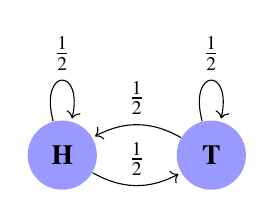
\begin{tikzpicture}
        % Add the states
        \node[state,
              text=black,
              draw=none,
              fill=blue!40!white] (s) {\textbf{H}};
        \node[state,
              right=of s,
              text=black, 
              draw=none, 
              fill=blue!40!white] (r) {\textbf{T}};

        % Connect the states with arrows
        \draw[every loop]
            (s) edge[bend right, auto=left]  node {$\frac{1}{2}$} (r)
            (r) edge[bend right, auto=right] node  {$\frac{1}{2}$} (s)
            (s) edge[loop above]             node  {$\frac{1}{2}$} (s)
            (r) edge[loop above]             node  {$\frac{1}{2}$} (r);
    \end{tikzpicture}
\end{figure}\\

From the transition matrix, we have 1 transient state and 2 absorbing states.\\ Q = $\begin{bmatrix} \frac{1}{4} \end{bmatrix}$ and R = $\begin{bmatrix} \frac{1}{4} & \frac{1}{2} \end{bmatrix}$
\begin{equation*}
\begin{split}
 N &= \brak{I - Q}^{-1}\\
 &= \brak{\sbrak{1} - \sbrak{\frac{1}{4}}}^{-1}\\
 &= \sbrak{\frac{4}{3}}
\end{split}
\end{equation*}
We know that probability of being absorbed by state j after starting in state i is given by the $\brak{i,j}^{th}$ entry of the matrix M, where M = NR.\\
M = $\begin{bmatrix} \frac{1}{3} & \frac{2}{3} \end{bmatrix}$.\\
 Hence the probability of being absorbed by state Y $\brak{1^{st} \text{element of R}}$ after starting with state $X_{1}\brak{1^{st}\text{element of Q}}$ is $M_{1,1}$\\
 \\
$\therefore \pr{Y}=\frac{1}{3}=0.33$ $\brak{\text{correct upto 2 decimal places}}$


\end{document}